In this Chapter, we detail the methodology adopted to perform formal verification of stand-alone solar PV systems using formal methods, more specifically model checking. Diagrams, flowcharts, and algorithms support and explain the solutions. The experimentation, case studies, and results are also presented. In addition, the Chapter contains a comparison with a specialized simulation tool, and also the use of different verifiers that evaluate performance by means of automated verification. Tables, commented reports, and graphic outputs are presented to aid  understanding.

Additionally, we present all assumptions and premises adopted, all of which support the results/conclusions, with direct impact on them. Usually, a premise is an unquestionable fact, however assumptions can be questioned. Unlike premises, assumptions are not explicit and need to be deciphered. With that in mind, we perform a detailed explanation of all assumptions over the course of the Chapter.

It is important to emphasize that the theoretical basis of the subject presented in this chapter was discussed in Chapter 1, ~\nameref{chap:background}. In addition, knowledge of the literature is essentila to aid understanding.


\section{Methodology for Automated Verification of Solar PV Systems}

Fig.~\ref{fig:validation} illustrates how a stand-alone solar PV project can be validated, starting with the traditional techniques - manual, simulation, testing, only then including the proposed automatic verification that is detailed in this Section. 

Note that, on the one hand, although the input information is the same for all the techniques, automated validation is different in that it is possible to define the bound $k$ to restrict the space-design search. Among the possible inputs are: weather data at the location (temperature, solar irradiance, and insolation); system sizing information regarding specifications and configuration of PV panels, charge controller, inverter, batteries, DC bus  voltage; and requirements (battery autonomy, electric load demand, electric peak power demand, energy consumption, load curve, and AC voltage).

In contrast, the outputs are not equal: design-space coverage and the information presented as result. Design-space coverage was shown in chapter \nameref{chap:background} to be the most complete when performed by automated verification, event using the bound $k$ to restrict the search, it not being necessary to unbound the system completely in order to discover a design flaw. Moreover, testing and simulation depend on the test vector used as input to evaluate the system.

With respect to the results presented, a project validated manually is just a piece of paper; simulation software produces success - fail information and can additionally present the optimized design if the system evaluated has some flaw, with graphics and reports; testing (whether laboratory or field) uses  measurement equipment and/or data from monitoring systems. Automated verification, as proposed in this thesis, presents success-fail information also, however the output is not graphic  (as will be shown), is summarized in reports with details about the variables and states of the project that cause a project flaw (in this case,  where a design flaw is detected).

\begin{figure}[h]
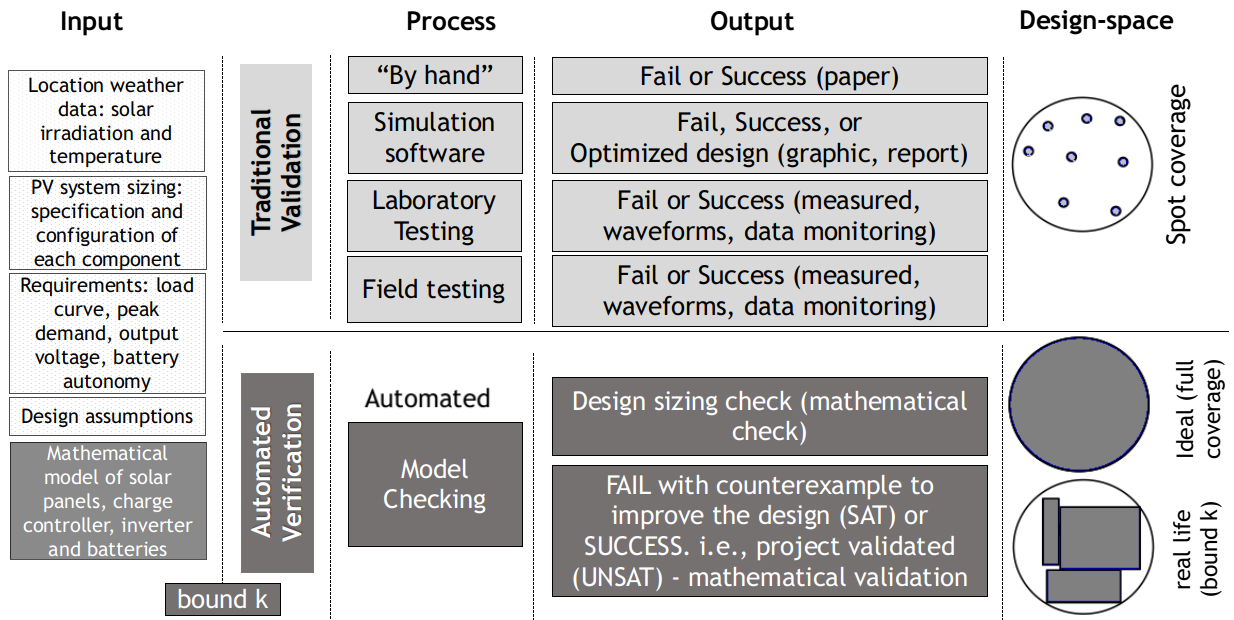
\includegraphics[width=1.0\textwidth]{PVprojectvalidation3g}
\centering
\caption{Project validation methods compared}
\label{fig:validation}
\end{figure}

Starting at this point, it will be shown how the proposed automated verification of stand-alone solar PV systems functions. 

The process begins with the conversion of a real PV system into a model. Fig. \ref{fig:systemverif} showed how a general system is converted to a model in order to be verified by model checking. Fig.~\ref{fig:systemverif4} is an adaptation of the general diagram, replacing the original system by a PV system and detailing the inputs, outputs, and requirements. 

It is important to bear in mind that the model checking process is the same whatever the system that is being validated; what is  important is to choose an accurate model, define the requirements/constraints, and get correct information from the system components, in order to achieve sound and effective validation.

\begin{figure}[h]
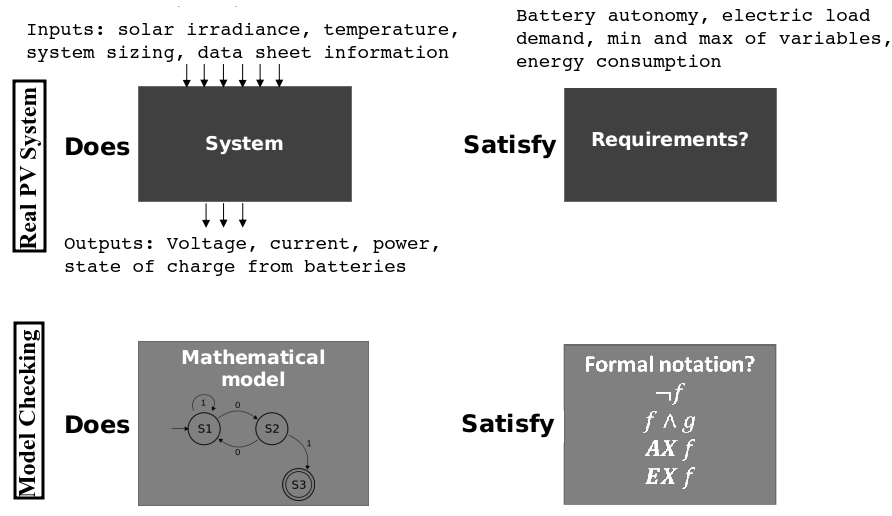
\includegraphics[width=0.8\textwidth]{systemverif4}
\centering
\caption{From real solar PV system verification to model checking. Source: adapted from \cite{Clarke2008}.}
\label{fig:systemverif4}
\end{figure}

The flowchart proposed for the automated verification method is illustrated in Fig.~\ref{fig:flowchartgeneral}. The three steps are the high level description of how the automated verification method can be used to validate solar PV systems.

\begin{figure}[h]
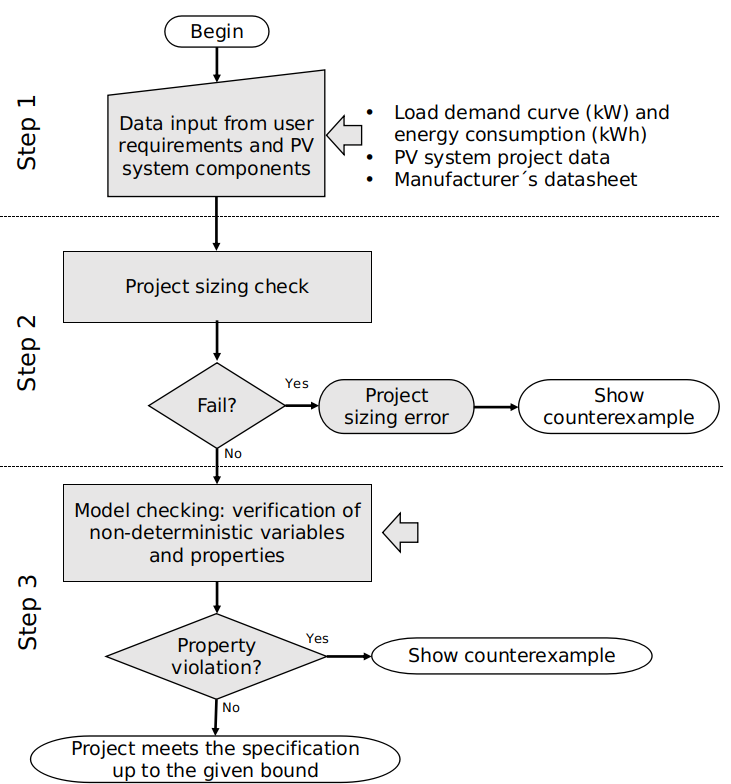
\includegraphics[width=0.6\textwidth]{flowchart_verification5.png}
\centering
\caption{Flowchart of the proposed automated verification of PV systems.}
\label{fig:flowchartgeneral}
\end{figure}

In \textbf{Step 1}, the PV input data %(e.g., load power demand and load energy consumption) 
and the formulae to check the sizing project, the mathematical model, the limits of the weather non-deterministic variables, are all written as an ANSI-C code~\cite{ANSI2018}. 

In \textbf{Step 2}, the sizing check of the PV system takes place: indicating if there is a sizing error before performing the automated verification of the system. This stage ensures that the system follows the standard project steps of the critical period method of sizing~\cite{Pinho}. 

\textbf{Assumption:} before the automated verification, which performs the verification of the intended system behavior, the sizing check of the system is performed. On the discover of an error, the process stops, showing the sizing error.

\textbf{Assumption:} The sizing check is performed using critical period criteria.

In \textbf{Step 3}, weather variables (e.g., solar irradiance and ambient temperature) will be systematically explored by our verification engine based on maximum and minimum values from the site where the PV system will be deployed. 
%As a consequence, all the formulae of the employed mathematical models will also be updated. 
In addition, depending on one of the desired properties of the system such as battery autonomy, energy availability, or even system power supply, our verification engine is able to indicate a failure if those properties are not met; in this particular case, it provides a diagnostic counterexample that shows in which conditions the property violation occurred. 
%; as the  state of charge of the batteries, load demand of power and the load consumption of energy if defined by the code
% (as reliability, performance, or safety)

%
%\textcolor{red}{In the following paragraph you should related the output of our verification engine with the description of the BMC SAT or UNSAR given above. For example, what does a failure mean? is it SAT?}
In short, the model checker will process the ANSI-C code with constraints ($C$) and properties ($P$) of the PV system, and the tool will automatically verify if the PV system requirements are met. If it returns a failure (i.e. SAT), then the tool provides a counterexample, i.e. a sequence of states that leads to the property violation; this information can be used as feedback to improve the PV system design. However, if the verification succeeds (i.e. UNSAT), there is no failure up to the bound $k$; therefore, the PV system will present its intended behavior up to the bound $k$.

%, i.e., our verification engine does not give any guarantee that there is no error in bound $k+1$ unless some induction method is employed~\cite{DBLP:journals/sttt/GadelhaIC17}.
%
%
%---------------------------------------------------------------------
% \subsection{The case studies and the Algorithm}
%---------------------------------------------------------------------
%
% 
%and as backup at night 
%
%The 700 W system: 3 x 325 W PV panels connected in series, controller of 150 V/35 A with a DC-bus of 24 V, 4 x 220 Ah batteries (2 in series and 2 in parallel arrangement), and inverter of 700 W. 
%
%And the 1,200 W PV system: 4 x 325 W connected in series PV panels, with controller of 150 V/35 A  in a DC-bus of 48 V, 4 batteries of 120 Ah connected in series, and a 1,200 W inverter.
%
%As demonstrated at this work, the performance of the system is highly dependent of solar irradiance and temperature, that are specific of the deployed local (latitude and longitude). 

Algorithm~\ref{alg:verification-algorithm} describes the equivalent pseudo-code. %Line 1 indicates a function call that performs the size checking of the each component of the PV system. %: using Equations \eqref{eq:NTPmin}, \eqref{eq:NTP}, \eqref{eq:NPSmin}, \eqref{eq:NPS}, \eqref{eq:NPP}, and \eqref{eq:NPPmin} to verify the PV panel; using \eqref{eq:Cbank}, \eqref{eq:Nbtotal}, and \eqref{eq:batcheck} to verify the batteries; using \eqref{eq:vcvsystem}, \eqref{eq:icmin}, and \eqref{eq:icicmin} to verify the charge controller; and using \eqref{eq:vindc}, \eqref{eq:voutac}, and \eqref{eq:invcheck} to verify the inverter. 
%The verification is carried out by the \textit{assert} macro from the ANSI-C programming language to encode each equation of sizing check. The argument to the \textit{assert} statement must be \textit{true} if the system specification is met; otherwise, the program aborts and prints a counterexample indicating a property violation. If there is no property violation, then the verification algorithm continues and 
In order to reduce the computational effort of the algorithm,
% caused by the state explosion inherent of the technique, 
every 24 h-day was considered as a time-step of 1 hour, and it was split into two parts: (a) one where PV generation is possible, during daylight, with a duration in hours depending on each site (but dependent on the sun and weather conditions); and (b) one that includes the rest of the day (with no PV generation), when the batteries are required to feed the house.

\textbf{Assumption:} The day is divided into two parts (representing presence or absence of PV generation, based on historical data from the location), considering average temperature and solar irradiance (for every hour of the day) and  annual insolation (per day).

Lines 1 carries information from the location where the PV system will be/was deployed. We use the average annual minimum and maximum, both for temperature ($T$) and solar irradiance ($G$), hour by hour, from~\cite{Temperature}, and ~\cite{Irradiance}.

\textbf{Premise:} Temperature, solar irradiance, and insolation data is available pertaining to the location where the solar PV system will be used.

Line 2 represents all the information that derives from the PV sizing and from the equipment manufacturer's data: PV, battery, inverter and charge controller specification and data. This item also includes information from the house's load curve.

\textbf{Premise:} The data sheet of every element of the solar PV system to be validated is available.

\textbf{Premise:} The detailed, sized project of the PV system is necessary in order to perform the validation (list of equipment and configuration, including voltage, current and how they are connected).

\textbf{Assumption:} The load curve of every house must be estimated or measured. Moreover, the time step is 1 hour, and seasonality is not considered, i.e. the load curve is the same for the entire year.

The first automated verification is the sizing check (line 3), if an error is found then the algorithm stops. In order to perform the sizing check, the algorithm uses Equations \eqref{eq:NTPmin}, \eqref{eq:NPSmin} and \eqref{eq:NPPmin} to verify the PV panel, Equations \eqref{eq:Nbtotal}, and \eqref{eq:batcheck} to verify the batteries, Equations \eqref{eq:vcvsystem}, \eqref{eq:icmin} and \eqref{eq:icicmin} to verify the charge controller; and Equations \eqref{eq:vindc}, \eqref{eq:voutac} and \eqref{eq:invcheck} to verify the inverter.

Then, if no sizing design flaw is found, two functions, called at lines 4 and 5, are responsible for discovering at which hour PV generation starts and when it stops. These functions receive this information from the array inputted to the Algorithm with the solar irradiance values.

The batteries are assumed to be charged, i.e. with SOC of 100\% (line 6).

\textbf{Assumption:} Batteries are considered charged at the start of project validation.

The first for-loop at line 7 controls how many 24 hours cycleswill be performed by the Algorithm.  And the for-loop from lines 8 to 11 is responsible for discharging the battery (according the load curve) and verifying the state of charge of the battery, hourly, from the first hour of the day after the sun sets to the next day before the sun rises (without PV generation). Then, at the next for-loop, from line 12 to 29, verification is performed where there is solar irradiance and the whole PV system works. The Algorithm generates information hourly related to average temperature ($T$) and solar irradiance ($G$), using non-deterministic variables from the model checker to explore all possible states and the \textit{assume} macro to constrain the non-deterministic values using a given range (lines 15 and 16). 
%and irradiance varies from 0 W/m$^{2}$ to 852 W/m$^{2}$ (with minimum of 274 W/m$^{2}$ during the daytime, when there is sunlight). 
%there is PV generation only between 8:00 h and 16:00 h every day, 
%with zero electric energy generation from 18:00 h to 6:00 h of the next day; and with insignificant generation from 6:00 h to 8:00 h, and from 16:00 h to 18:00 h of the same day. 

After that, the model of the PV generator is used in the function call of line 17, to produce the voltage and current considering the states of $G$ and $T$. With respect to every hour considered, the conditional \textit{if-elseif-endif} statements from lines 18, 20, 22, 24 and 26, will imitate the charge controller's work, as depicted in Table~\ref{table:controller} of Section~\ref{sec:controller}, performing the charge or discharge of batteries according to the value of the different variables: if there is PV generation, the updated battery state of charge, the house's load and the PV system set-up information.

At the end of the last for-loop, the state of the batteries is verified again (line 27) and the hour is adjusted to the next loop (line 28).

Nevertheless, if the verification engine does not fail, we can conclude that the PV system does not need further corrections up to the given bound $k$.
%
%\textcolor{red}{this sentence is unclear... After this process is started the battery autonomy verification, from line 31}. \textcolor{red}{this sentence is unclear... Based on the fact that won't be PV generation after a given time of the day, the algorithm will only discharge the batteries until a new charging process (at the next day) to start.} \textcolor{red}{what do you mean by The formal verification is guaranteed?...  The formal verification is guaranteed by  macro to specific variables of the model, according lines 27 and 35.}
% and the non-deterministic variables $G$ and $T$ are considered during the formal verification of the system, otherwise, during the other two periods, there is no PV generation and just the power consumption from the backup batteries. 
%Within this 8h-period, $G$ and $T$ are automated verified with different values every one hour.
%, and change their value every 1 h according with the algorithm created using the technique.
 \begin{algorithm}
 \caption{Model checking algorithm for validation of stand-alone PV systems}
 \begin{algorithmic}[1]
 \begin{scriptsize}
 \renewcommand{\algorithmicrequire}{\textbf{Input:}}
 \renewcommand{\algorithmicensure}{\textbf{Output:}}
 \REQUIRE mathematical model (PV, batteries, inverter, charge controller), weather data (temperature, solar irradiance), system sizing details, design requirements (load curve, peak demand, output voltage, battery autonomy), design assumptions (system availability, battery state of charge, 1-hour step of validation)
 \ENSURE design sizing check; FAIL with counterexample to improve the design; SUCCESS, saying that the project has no flaws
  \STATE $declare \, min \, and \, max \, solar \, irradiance[24h], \, and \, temperature[24h]$\\
  \STATE $declare \, case \, studies \, details: \, sizing \, and \, manufacturers \, data $ \\
  \STATE $sizing \_ check()$ \\
  \STATE $startPVgeneration \leftarrow findStartPVgeneration()$ \\
  \STATE $endPVgeneration \leftarrow findEndPVgeneration()$ \\
  \STATE $SOC \leftarrow 100\%$ \\
%  \COMMENT {Starting with the PV generation time}
% \\ 
%\textit{LOOP Process}
 \FOR {$1st \, 24h \, loop$ to $Nth \, 24h \, loop$}
  \FOR {$endPVgeneration+1$ to $startPVgeneration-1$}
	  \STATE $dischargeBattery \, in \, 1h()$ \\
%	  \STATE $autonomyCount \leftarrow autonomyCount+1$ \\
	  \STATE $assert (SOC \geq SOC \_ min)$ \\
%	  \STATE $battery \, autonomy \, verification()$ \\
  \ENDFOR
  \FOR {$startPVgeneration$ to $endPVgeneration$}
    \STATE $G \leftarrow nondet \_ uint(\,)$ \COMMENT {$G$ is non-deterministic variable}
    \STATE $T \leftarrow nondet \_ uint(\,)$ \COMMENT {$T$ is non-deterministic variable}
    \STATE assume ($Gmin \leq G \leq Gmax$) \COMMENT {restricting $G$ values}
    \STATE assume ($Tmin \leq T \leq Tmax$) \COMMENT {restricting $T$ values}
    \STATE $Imax, Vmax \leftarrow PVgenerationMODEL (G,T)$ \\
    \COMMENT {If-then-else sequence to imitate charge controller work}
    \IF {($battery \, is \, empty$) AND ($PV \, is \, generating$)}
      \STATE $chargeBattery \, in \, 1h()$ \COMMENT {PV feed the house}
    \ELSIF {($battery \, is \, empty$) AND NOT($PV \, is \, generating$)}
      \STATE FAIL with assert macro \COMMENT {Battery is empty and there is not PV generation}
    \ELSIF {NOT($battery \, is \, empty$) AND ($PV \, is \, generating$)}
      \STATE stop battery charge \COMMENT {PV feed the house}
    \ELSIF {NOT($battery \, is \, empty$) AND NOT($PV \, is \, generating$)}
      \STATE $dischargeBattery \, in \, 1h()$ \COMMENT {Battery feed the house}
    \ENDIF
    \STATE $assert (SOC \geq SOC \_ min)$ \\
    \STATE $hour \leftarrow hour+1$ \\
   \ENDFOR
  \ENDFOR
 \RETURN $(\,)$ 
  \end{scriptsize}
 \end{algorithmic} 
 \label{alg:verification-algorithm}
 \end{algorithm}

%\subsubsection{Assumptions and Premises} 
%

\section{General Assumptions}
\label{sec:assumptions}

In order to be clear, we now provide a list of the assumptions adopted by the scientific automated verification methods developed in this thesis.

The code in ANSI-C, was created to perform both methods, automated verification and automated synthesis, regardless of the verifier used. This means that: 

\begin{itemize}
\item The `\# include' preprocessor directive is not used, despite being very common in the C language, which allows the use of C language libraries, including the mathematical one;
\item In the absence of the `\# include' directive, it was necessary to create specific mathematical functions at the proposed code in order to calculate the exponential `$exp(x)$' or $e^{x}$, and natural logarithm `$log(x)$' functions, used for the solar PV model;
\item There is no `\# define' preprocessor directive. Therefore, global variables were used to replace it;
\item The macro `assert (expression);' must be replaced by `if (!expression) \{ \_ \_ VERIFIER\_ error();\}';
\item The macro `assume (expression);' must be replaced by `\_ \_ VERIFIER\_ assume(expression);';
\item It is not possible to use the \# if, \# else, \# elif, \# endif or \# ifdef, \# ifndef commands.
\end{itemize}

Regarding the automated verification scientific method:

\begin{itemize}
\item A value of bound $k$ was used to restrict the design-space and improve performance. The choice of value was empirical, following tests with the code;
\item All the PV system model, user requirements, assumptions, and technical information from the PV system equipment are written as an ANSI-C code.
\end{itemize}

Of the off-the-shelf simulation tools, only HOMER Pro and Hybrid2 perform off-grid system with battery backup analysis. Additionally, HOMER and RETScreen include economic analysis or even optimization-sensitive analysis; however RETScreen does not have the capacity for stand-alone solar PV system analysis. Therefore, in this study, HOMER Pro will be the only simulation tool used to compare with our method.  

For all case studies, the minimum battery state of charge was defined at $75$\%, and the efficiency of $86$\%, which is common to lead-acid batteries (adopted as standard here), and the AC voltage from the inverter at $127$ V (Brazilian standard). According with the evaluated local of the PV systems installation, the considered insolation for the worst month is $3.8 kWh/m^{2}$ per day.


\section{Description of the Case Studies}
%------------------------------------------

%We have performed five case studies to evaluate our proposed verification method: (a) four PV systems (three in series 325W PV panels, four 220 Ah batteries in a configuration with two series and two parallel with 48h autonomy, 700 W inverter with peak power of 1,600W, charge controller with MPPT with 35A/150V of capacity) deployed in four different houses in an indigenous community (GPS coordinates 2$^{o}$44'50.0"S 60$^{o}$25'47.8"W) situated nearby Manaus (Brazil), with each house having a different power demand (house 1 = 253 W, house 2 = 263 W, house 3 = 283 W, and house 4 = 501 W); and (b) one case concerning a system deployed as an individual system in Manaus (GPS coordinates 3$^{o}$4'20.208"S 60$^{o}$0'30.168"W), supporting 915 W of the house's load (house 5 with four 325W PV panels in a configuration two series and two parallel, four 120Ah batteries in series and autonomy of just 6 h, 1,200 W inverter with surge of 1,600 W, charge controller with MPPT of 150V/35A). 
Five case studies evaluated the proposed approach, as described in Table~\ref{tab2}. %Furthermore, three start-of-art verification tools, as described in Section~\ref{sec:AutomatedVerification} (ESBMC, CBMC, and CPAchecker), and HOMER Pro simulation tool were used to compare the approach effectiveness and efficiency.
These case studies were defined based on the usual electrical load found in riverside communities in the State of Amazonas,  Brazil~\cite{TrindadeCordeiro19, Agrener2013}.

It is important to mention that the load curve represents an array of $24$ integer numbers, one for each hour of the day (instant power in Watts) and it was estimated after visits to the communities and a survey applied in June $2017$, before the houses were electrified.

\begin{table}
\caption{Case studies: stand-alone solar PV systems.}\label{tab2}
\begin{scriptsize}
\begin{tabular}{|c|c|c|c|c|c|}
\hline
\hline
Item & House 1 & House 2 & House 3 & House 4 & House 5\\
\hline
\hline
PV Panels &  \multicolumn{4}{|c|}{3$\times$325 W: (3S)} & 4$\times$325 W: (2S-2P) \\
\hline
Batteries & \multicolumn{4}{|c|}{\makecell{4$\times$220 Ah: (2S-2P)\\ autonomy: 48 h}} & \makecell{4$\times$120 Ah: (4S)\\ autonomy: 6 h}\\
\hline
Charge Controller & \multicolumn{5}{|c|}{With MPPT of 150 V/35 A}\\
\hline
Inverter & \multicolumn{4}{|c|}{700 W, surge: 1,600 W} & 1,200 W, surge: 1,600 W\\
\hline
Load power peak (W)& 342  & 253  & 263 & 322 & 814 \\
\hline
Load Power surge (W)& 342 & 722 & 732 & 896 & 980\\
\hline
Load curve (W) & \multicolumn{5}{|l|}{\makecell{House 1: 118-118-118-46-46-46-95-95-170-170-296-242-242-95-95-95-95-95-342-288-288-288-288-118\\House 2: 136-136-136-136-136-136-67-67-184-184-184-184-184-67-67-67-67-67-253-253-253-253-253-136\\House 3: 113-113-113-113-113-113-67-67-217-97-97-97-97-97-97-97-97-97-263-113-113-113-113-113\\House 4: 207-207-207-135-135-135-66-66-161-161-233-253-248-66-66-66-66-66-302-317-322-302-302-207\\House 5: 45-16-16-16-16-16-0-0-0-72-72-222-150-150-0-0-72-72-814-814-814-742-742-16}}\\
\hline
\makecell{Consumption\\ (kWh/day)}& 3.9 & 3.6 & 2.5 & 4.3 & 4.88\\
\hline
GPS Coordinates & \multicolumn{4}{|c|}{\makecell{2$^{o}$44'50.0"S 60$^{o}$25'47.8"W\\}} & \makecell{3$^{o}$4'20.208"S \\60$^{o}$0'30.168"W}\\
\hline
Details & \multicolumn{4}{|c|}{\makecell{Riverside indigenous community\\Rural Area of Manaus - Brazil}} & \makecell{Urban house \\Manaus-Amazonas-Brazil}\\
\hline
\hline
\end{tabular}
Caption: (S): Series; (P): Parallel.
\end{scriptsize}
\end{table}

%------------------------------------------
\section{Objectives and Setup}
\label{sec:setup}
%------------------------------------------

The experimental evaluation aims to answer two experimental questions:
%
\begin{enumerate}
\item[EQ1] \textbf{(soundness)} Does the automated verification approach provide correct results?
\item[EQ2] \textbf{(performance)} How do the verifiers compare to each other and to a commercial simulation tool?
\end{enumerate}

%In order to evaluate the proposed verification method and its performance, we have considered five case studies, three verification engines in different configurations, and also compared the results to the HOMER Pro tool. All the experiments were performed with a time out of 14,400 seconds. %Every dweller, who owns a PV system, was interviewed 
%
All experiments were conducted on an otherwise idle Intel Xeon CPU E5-4617 (8-cores) with 2.90 GHz and 64 GB RAM, running Ubuntu 16.04 LTS 64-bits. The setup of HOMER Pro v3.13.1 was an Intel Core i5-4210 (4-cores), with 1.7 GHz and 4 GB RAM, running Windows 10. The experiments were performed with a time out of 240 minutes.

The verification engine ESBMC, version v6.0.0 was used with the SMT solver Boolector version 3.0.1~\cite{Brummayer}\footnote{Command-line: \$ esbmc filename.c -\phantom{}-no-bounds-check -\phantom{}-no-pointer-check -\phantom{}-unwind 100 -\phantom{}-boolector}; and an alternative ESBMC v6.0.0 was used with the 'incremental SMT' mode\footnote{Command-line: \$ esbmc filename.c -\phantom{}-no-bounds-check -\phantom{}-no-pointer-check -\phantom{}-unwind 100 -\phantom{}-smt-during-symex -\phantom{}-smt-symex-guard -\phantom{}-z3} enabled; with SMT solver Z3 version 4.7.1~\cite{DeMoura}. % with the goal of reducing memory usage.

The verification engine CBMC 5.11 and MiniSat 2.2.1 were used in the comparison~\cite{Kroening}\footnote{Command-line: \$ cbmc filename.c -\phantom{}-unwind 100 -\phantom{}-trace}.
 
The verification engine CPAchecker 1.8 was used \footnote{Command-line: \$ scripts/cpa.sh -heap 64000m -stack 10240k -config config/bmc-incremental.properties -spec config/specification/sv-comp-reachability.spc filename.c}, with the SMT solver MathSAT version 5.5.3~\cite{mathsat5}. An alternative CPAchecker configuration was also tried, using the BMC k-induction option, but the results show no improvement in performance or soundness (so it is not reported here).

%\section{Verifiers Environment}
%\label{sec:verifenviron}

%------------------------------------------
\section{Experimental Results and Discussion}
\label{sec:results_indeed}
%------------------------------------------

This Section presents the results, with commented outputs produced by every tool, mainly related to the reports (CBMC and ESBMC) and some graphic resources (CPAchecker and ESBMC).

%\textcolor{red}{We should answer the two% research questions here... please take a look at https://ssvlab.github.io/lucasccordeiro/papers/cav2017.pdf to check how you can answer.}
%\begin{enumerate}
%\item[RQ1] \textbf{(soundness)} Does our approach provide correct results?
%\item[RQ2] \textbf{(performance)} How does our approach compare against other existing tools?
%
Table~\ref{cases} summarizes the results. The times reported in Table~\ref{cases} answer EQ2. 
Note that an UNKNOWN result from the proposed verification engines does not mean that a failure was found nor that the verification was successful: it indicates that the verification engine led to an \textit{out of memory} or a \textit{time out} situation.

%HOMER Pro result: the $1,200$W was the only one that was proved to not meet the requirement of battery autonomy; all the 700W systems had no indication of flaws during simulation. The simulation took less than five seconds to be performed on each case study.
%
\begin{table}
\centering
\caption{Summary of the case-studies comparative and the automated tools.}\label{cases}
\begin{scriptsize}
\begin{tabular}{|c|c|c|c|c|}
\hline
\hline
\multicolumn{5}{|c|}{Model Checker (SAT/UNSAT: time and message)}\\
\hline
Case &  \makecell{ESBMC 6.0.0\\(Boolector 3.0.1)} & \makecell {ESBMC 6.0.0\\(Z3 4.7.1)} & \makecell{CBMC 5.11\\(MiniSat 2.2.1)} & \makecell{CPAchecker 1.8\\(MathSAT 5.5.3)}\\
\hline
\hline
House 1 &  \makecell{Out of memory \\(UNKNOWN)} & \makecell{05 m 08 s \\(UNSAT)} & \makecell{19 m 02 s \\(UNSAT)} & \makecell{Time out \\ (UNKNOWN)}\\
\hline
House 2 &  \makecell{Out of memory \\(UNKNOWN)} & \makecell{04 m 27 s \\(UNSAT)} & \makecell{18 m 59 s \\(UNSAT)} & \makecell{Time out \\ (UNKNOWN)}\\
\hline
House 3 &  \makecell{Out of memory \\(UNKNOWN)} & \makecell{05 m 07 s \\(UNSAT)} & \makecell{18 m 39 s \\(UNSAT)} & \makecell{Time out \\ (UNKNOWN)}\\
\hline
House 4 &  \makecell{Out of memory \\(UNKNOWN)} & \makecell{04 m 37 s \\(UNSAT)} & \makecell{18 m 36 s \\(UNSAT)} & \makecell{Time out \\ (UNKNOWN)}\\
\hline
House 5 &  \makecell{Out of memory \\(UNKNOWN)} & \makecell{$\leq$ 1 sec \\(SAT Line 337)} & \makecell{$\leq$ 1 sec \\(SAT Line 337)} & \makecell{6 sec \\ (SAT line 337)}\\
\hline
\hline
\end{tabular}
\end{scriptsize}
\end{table}

The description of the experimental results have been broken down into three parts, one for each verification engine: ESBMC, CBMC, and CPAchecker. 

\subsection{ESBMC}
\label{sec:ESBMCverification}

Two alternatives were tested with ESBMC: one with Boolector and the another with Z3. The 'incremental SMT' option, which uses less memory, can be performed with Z3 only since ESBMC does not support the 'incremental' mode with the Boolector solver yet. 

Using ESBMC with Boolector led to an out of memory situation in all the case studies. This result was obtained in less than six minutes of execution, i.e. the $64$ GB of RAM were consumed by the verification engine and the processes were killed, thus leading to an UNKNOWN result returned by ESBMC as shown in the first column of Table~\ref{cases}. 

However, running the same version of ESBMC, using 'incremental SMT' solving with Z3, the experimentation results returned were conclusive (SAT or UNSAT) in all the case studies. 

In the houses that use a $975$ W PV system (house $1$, house $2$, house $3$, and house $4$), ESBMC could not reach an error in any of the four houses and the execution time took from $04$ m $27$ s to $05$ m $08$ s. Fig.~\ref{fig:esbmcverifhouse1} shows the output report of the tool for house $1$, with the absence of fail at the end of the analysis. The file produced by ESBMC is $160$ lines long and $12.4$ kB in size. The author highlighted the result, which shows that no design flaws were found (SAT result or SUCCESS) within the bound $k$ of $100$.

\begin{figure}[h]
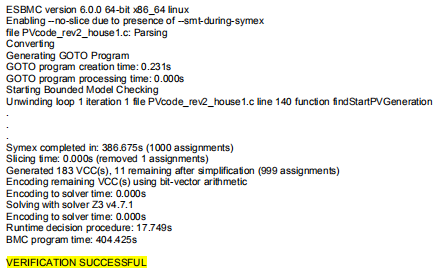
\includegraphics[width=0.65\textwidth]{esbmcverifh1.png}
\centering
\caption{Report generated by ESBMC (with Z3 solver) after validation of House 1.}
\label{fig:esbmcverifhouse1}
\end{figure}

However the $1,200$ W PV system (house $5$) failed (SAT) in line $337$ of the code, thereby indicating that the system is \textit{incorrectly} sized; in particular, the counterexample provided by the verification engine indicated that the nominal current from the charge controller is less than the minimum current required by the PV system, indicating that the equipment chosen is not suited to meet the design requirements.

Fig.~\ref{fig:esbmcverifhouse5} shows the report generated by the tool, with red highlights for the result, showing the incompatibility of the sized charge controller and the minimum necessary. The report generated by ESBMC was a text file of $14.1$ kB in size, $353$ lines in length. This verification took less than $1$ s to perform, as indicated in the last line of Table~\ref{cases}, faster than the previous analysis because ESBMC stops during the sizing check, line $3$ of Algorithm~\ref{alg:verification-algorithm}, and does not perform the rest of the verification code.

\begin{figure}[h]
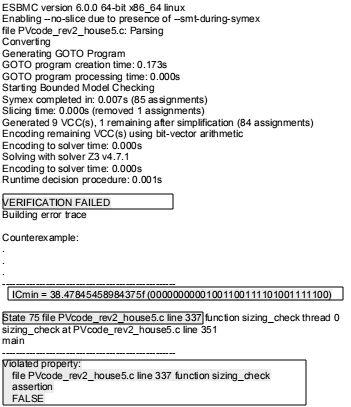
\includegraphics[width=0.5\textwidth]{esbmcverifh5.png}
\centering
\caption{Report generated by ESBMC (with Z3 solver) after validation of House 5.}
\label{fig:esbmcverifhouse5}
\end{figure}

%At the terminal, the command used to perform the verification is:
%\$ esbmc filename.c -\phantom{}-no-bounds-check -\phantom{}-no-pointer-check -\phantom{}-no-div-by-zero-check -\phantom{}-unwind 300 -\phantom{}-smt-during-symex -\phantom{}-smt-symex-guard --z3
%
%Where:
%
%\begin{itemize}
%\item The first three parameters, after the filename, are related to options that are usual to find bug in software, %for example, like bound check to arrays, pointer check, and division by zero, 
%but unnecessary to check at this kind of problem (if not removed, there is lost of performance during the automated verification);
%\item The parameter $unmind$ tells to ESBMC the limit to unroll the loops. This number was optimized (empirically) in order to reduce the running time and avoid to unwind unnecessarily the loops;
%\item The two parameters with $symex$ tell to ESBMC to perform an incremental SMT solving. There are other options, but this parameter is necessary because the complexity of the algorithms. The incremental SMT solving uses few RAM memory, compared with other SMT solving. 
%During empirical tests of the algorithms, the incremental solving was the only one who do not demanded 100\% the RAM memory. The use of swap-memory, i.e., the use of hard disk, reduces the performance and must be avoided;
%\item And the last parameter says to the tool that the Z3 SMT solver will be used.
%\end{itemize}
%

\subsection{CBMC}

Similar results were obtained with the CBMC tool, but with slower times than with ESBMC. The experimentation returned SAT or UNSAT for all the case studies, i.e. it was conclusive for all houses. 

In the $975$ W PV systems (house $1$, house $2$, house $3$, and house $4$), the tool could not reach an error in any of the four houses in an execution time of $18$ m $36$ s to $19$ m $02$ s. 

Fig. \ref{fig:cbmcverifhouse1} shows part of the report produced by CBMC when validating house 1. This file contains $270,512$ lines and is $39$ MB in size. The author highlighted the result, which shows that no design flaws were found within the bound $k$ of $100$.

\begin{figure}[h]
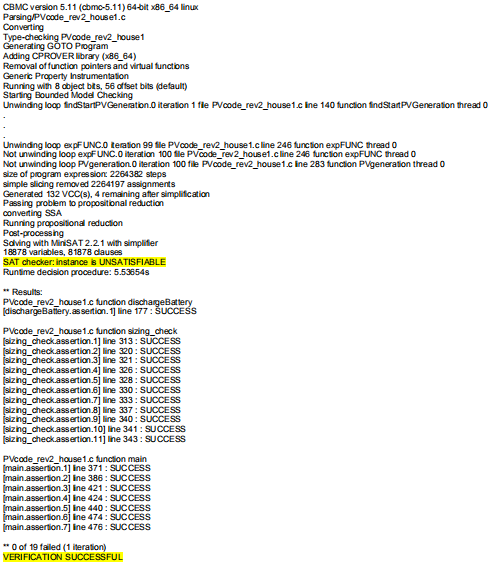
\includegraphics[width=0.8\textwidth]{cbmcverifh1.png}
\centering
\caption{Report generated by CBMC after validation of House 1.}
\label{fig:cbmcverifhouse1}
\end{figure}

However, the $1,200$ W PV system (house $5$) failed (SAT) in line $337$ of the code; with the same counterexample presented by ESBMC. This verification also took less than $1$ s to perform. Fig.~\ref{fig:cbmcverifhouse5} shows the (edited) report produced, with highlights on the flaw found: the minimum controller current needed for the PV systems is not compatible with the chosen controller of the sized system. The report file generated contains $217$ lines and was $13$ kB in size.

\begin{figure}[h]
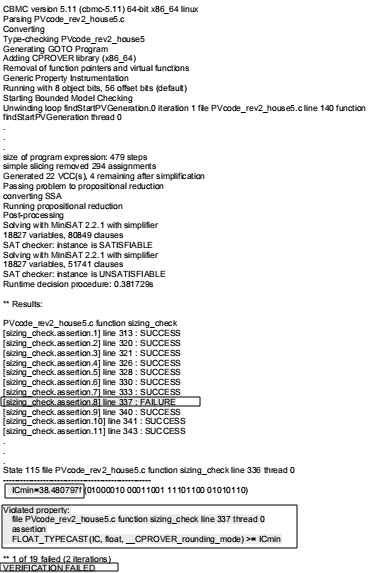
\includegraphics[width=0.7\textwidth]{cbmcverifh5.png}
\centering
\caption{Report generated by CBMC after validation of House 5.}
\label{fig:cbmcverifhouse5}
\end{figure}


\subsection{CPAchecker}
%\label{sec:CPAresult1}

Finally, the CPAchecker tool presented some different results. Even using two different configuration possibilities, as described in Section~\ref{sec:setup}, the verification engine presented an UNKNOWN result for all the $975$ W systems (house $1$, house $2$, house $3$, and house $4$). 

This is because the \textit{time out} limit was reached, i.e. after $4$ hours of execution the tool was unable to decide if the verification was SAT or UNSAT. This is shown in Fig.~\ref{fig:cpavalidh1} which reproduces one of the text reports issued by CPAchecker. Unlike ESBMC and CBMC, CPAchecker produces many different reports, notably for log, statistical, and counterexample files (which are in graphic, not text format).

\begin{figure}[h]
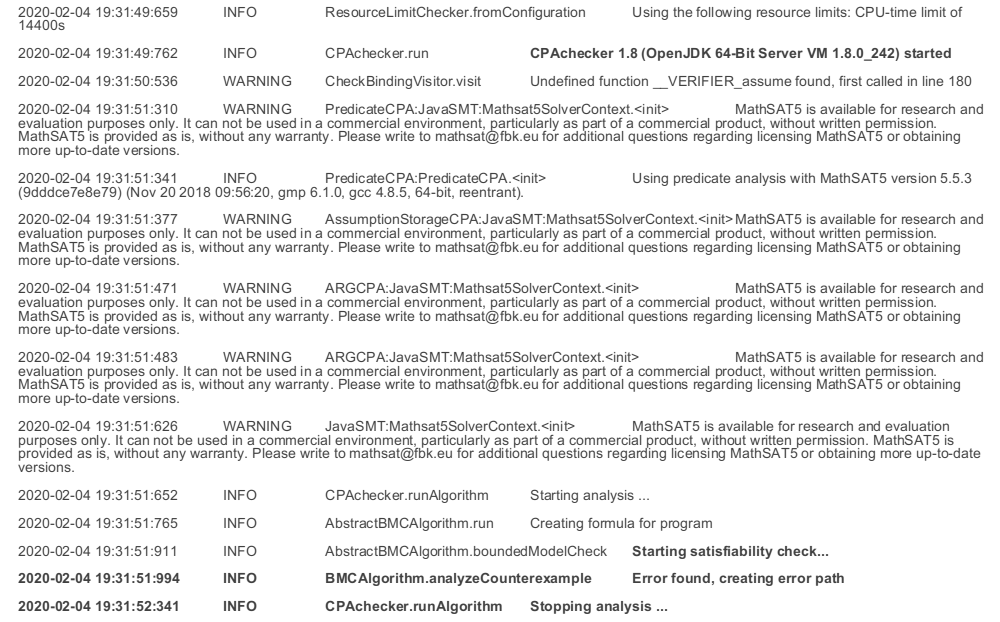
\includegraphics[width=0.8\textwidth]{CPA_verif_h1.png}
\centering
\caption{CPAchecker time out result for house 1 validation (file CPALog.txt).}
\label{fig:cpavalidh1}
\end{figure}

However, when validating the $1,200$ W PV system (house $5$), the tool presented the same SAT produced by the other engines, but with an execution time of $6$ seconds. Fig.~\ref{fig:cpavalidh5} shows the result, with highlights on the line that causes the fail ($IC_{min}$) and part of the CFA (control-flow automata, represented as a control-flow graph) diagram pointing to this fail.

\begin{figure}[h]
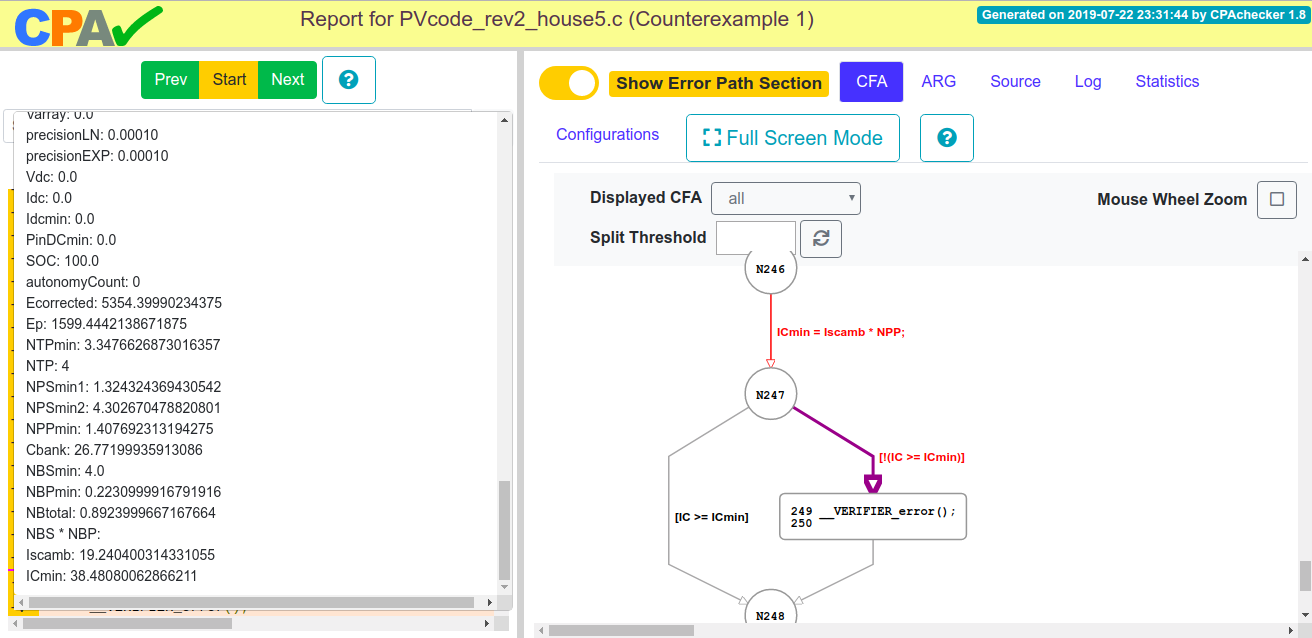
\includegraphics[width=1.0\textwidth]{CPA_verif_h5.png}
\centering
\caption{CPAchecker time out result for house 5 validation (file Counterexample.html).}
\label{fig:cpavalidh5}
\end{figure}


\subsection{HOMER Pro Specialized Simulation Tool}
\label{sec:homerenviron}

HOMER Pro is a powerful specialized electrical systems simulator, however even with the simulation characteristic, it performs optimization only when a given design is inputted to the schematic of the tool. This means that HOMER does not maintain the characteristic of the system under evaluation. It starts with the inputted information, but uses the optimization default set up to increase or decrease the characteristic of each component until the load is fulfilled by the electrical generation system, and at the lowest cost. 

Therefore, in order to perform a limited simulation and not exceed the values of each component (for example, the total power of the PV array under evaluation), the `search space' must be used for sizing instead of the `HOMER Optimizer'. This is done on the menu of each component inputted in the schematic of the tool. 

The PV panels and batteries: simulation of a particular capacity for PVs and batteris is possible using the `search space' for sizing instead of the `HOMER Optimizer'. It is possible either to aggregate all the PV panels as a single PV component, in which case, the search space must vary from 0 to 1, i.e. from the option without PV panels until it reaches the power inputted to the component in the HOMER schematic, or add each PV component to represent the series' configuration. For the batteries, it is necessary to find the equivalent capacity of the series and parallel configuration since HOMER considers only one battery component per simulation even if multiple battery components are added to the schematic.

Another drawback of HOMER Pro is the fact that the user cannot set battery autonomy, as the HOMER controller will decide when it is economical to discharge the batteries during the simulation year. It follows that simulation of battery autonomy cannot to be evaluated.

As part of the comparison proposed, four $975$ W PV systems (houses $1$, $2$, $3$ and $4$) were evaluated by HOMER Pro (EQ2). The simulation results showed that for each of the sized systems, HOMER Pro concluded that no viable solution was found with the components inputted in the schematic. Fig. \ref{fig:homersimuh2no} shows one of the screens presented by HOMER Pro software, specifically by house $2$.

\begin{figure}[h]
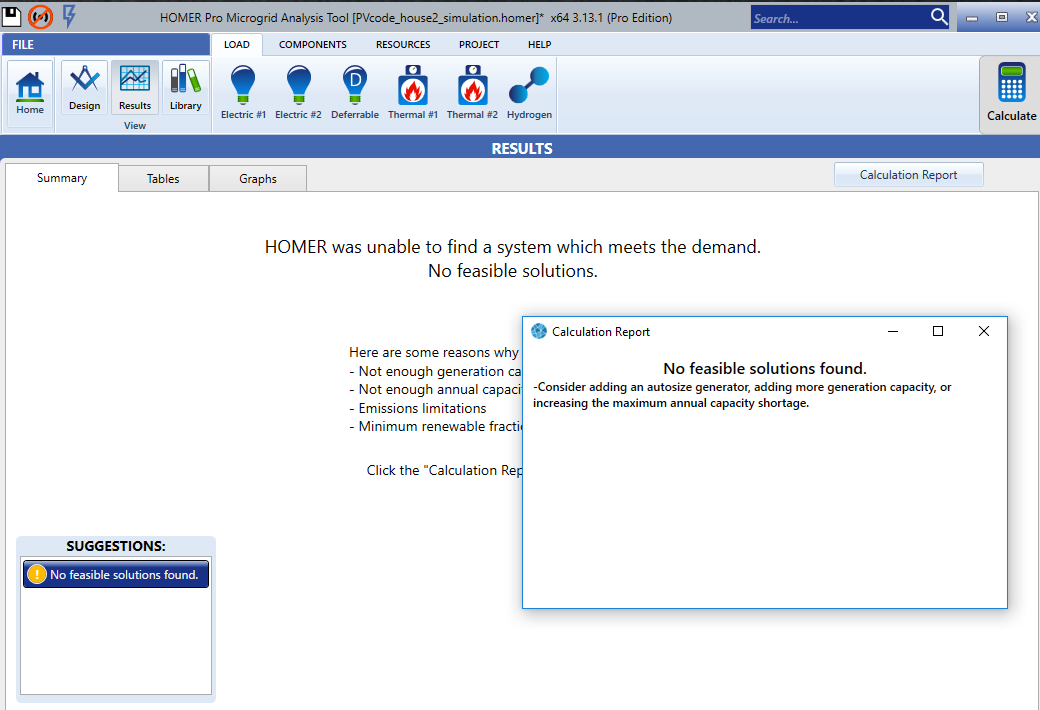
\includegraphics[width=0.8\textwidth]{homersimuh2no.png}
\centering
\caption{HOMER simulation screen presented for house 2 with no feasible solution found.}
\label{fig:homersimuh2no}
\end{figure}

Moreover, in order to evaluate the problem associated with the lack of a viable solution, some empirical changes were made to the  project under evaluation. Fig.~\ref{fig:homersimuh2yes} shows that a configuration with higher battery capacity (3 strings of 2 batteries each, 2S-3P, of 220 Ah; instead of 2 strings of 2 batteries each as in the original sized system) can solve the problem of house 2. The same is true of the other three houses of $975 W$, when improved battery capacity is presented by HOMER Pro as an optimal solution.

\begin{figure}[h]
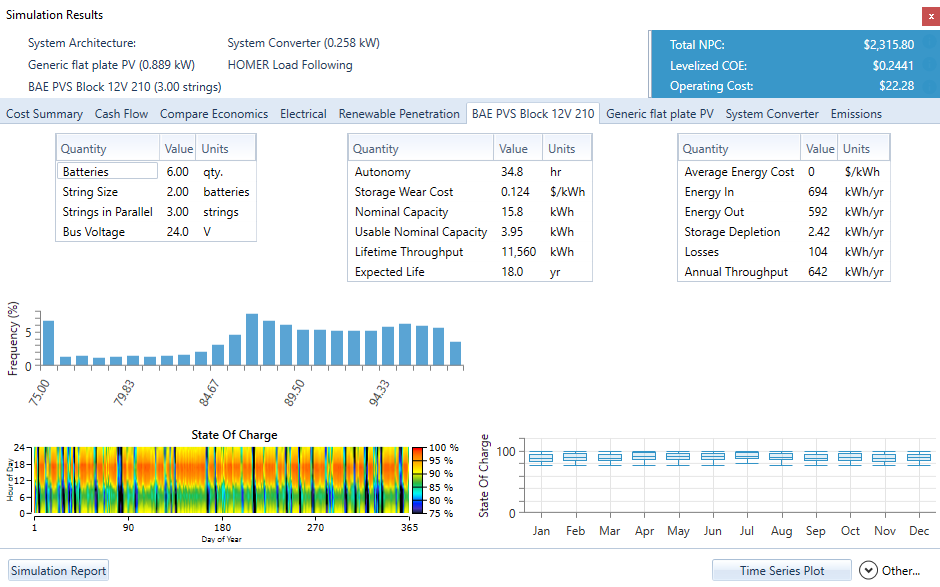
\includegraphics[width=0.8\textwidth]{homersimuh2yes.png}
\centering
\caption{HOMER simulation screen presented for house 2 with viable solution.}
\label{fig:homersimuh2yes}
\end{figure}

The case study that was not possible to simulate was the $1,200$ W (house $5$). The reason is that HOMER Pro does not allow battery autonomy setup (because it always sizes and optimizes the electrical system in order to meet the load requirements for an entire year of simulation); therefore, it was not possible to obtain any indication about the failures of this specific PV system with simulation (EQ2).  

%
%Note that a PV design always uses daily average values of sun hours to each site, with impact in the PV components. Those hours are based on historical data and, in field, it is not unusual to find days where that number of hours was not reached due to weather conditions. The season has impact since the case studies are from the rain forest, where clouds are always present. As a result, the identified flaws in houses 1, 2, 3, and 4, are justified once again.
%
%We have evaluated five case studies in total using the HOMER Pro tool and our automated verification tool. Related to the HOMER Pro, the simulation, based on NASA data from the deployed systems (temperature and solar irradiance), shows that the restrictions were met by four 700 W PV systems (house 1, 2, 3 and 4), without any indication of sizing error or even performance. The case study that was unsuccessful during simulation was the 1,200 W (house 5); however, without any indication about the failures of this PV system. All the simulations took less than 5 seconds (each) to be performed.
%
%However, related to the results of the automated verification: (a) the 1,200 W PV system (house 5) failed during the sizing check. The number of panels was \textit{incorrect}; in particular, the counterexample provided by our verification method indicated 3 panels in parallel and the sized project has 2 in series and 2 in parallel. That verification took 63.3 hours to be performed. Surveying the owner of the 1,200 W system it was identified that, in fact, the system mostly of the time do not met the battery autonomy (mainly when all the loads are turned on). That behavior is expected because the system was purchased as an off-the-shelf solution and not as a specific design for the electrical charges of the house; (b) Related to the four 700 W PV systems, just one verification finished its analysis (house 1) considering the time-out of 432 h of computing. The sizing check was successful during automated verification, but there was found flaw related with the battery autonomy, when SOC reached levels below of 75\%. The automated verification identified the flaw right after the first night-discharge cycle, before the solar system start to recharge the batteries. The proposed tool took 409.3 hours to find this error at house 1. This possible flaw was confirmed with the dweller that uses the system: at least once or twice a mouth is usual the system to turn off, normally during raining days or with more clouds in the sky, and after the sun rises the system returns to normal operation. Related to houses 2, 3 and 4, it was considered that the automated verification had a time-out condition, with no conclusive results.

\subsection{Comparing Automated Verification and Simulation Results with Real PV Systems}

Results diverged for houses $1$, $2$, $3$ and $4$ with respect to the proposed approach: the automated evaluation shows there is no project flaws, but simulation demanded improvement of battery capacity (adding one more string of batteries to the system). 

In order to evaluate which validation is correct, it was necessary to consult the access interviews conducted with the residents of the deployed systems. From July $2018$ to March $2019$, surveys were applied to the residents on a monthly basis and data was collected from a local monitoring system: energy interruptions of the PV systems were not reported every month. 

However, even when only one interruption is reported in a month, this represents around $3.33$\% interruption for the entire period ($1/30$), which indicates $96.97$\% of availability of the PV system ($96.67\% = 100\%-3.33\%$), and in accordance to what was described in Section~\ref{sec:availability}, the type of electrical load of the houses is not critical; this situation is considered an energy interruption, not a system flaw, further affirming EQ1. Therefore, the proposed approach using automated verification provides the correct evaluation of the PV system, thus answering EQ2.

All tools indicated flaws in house $5$ (automated verification or simulation); however, only the automated verification approaches indicated which design error was responsible for the flaw (charge controller specification), further answering EQ2.

In order to validate the possible flaw identified by the automated verification in house $5$, the owner of the $1,200$ W system was interviewed. From this it became clear that, in fact, the system does not meet the battery autonomy when all loads are turned on, and this was double-checked against the monitoring system of the charge controller, which showed that the maximum power or surge power was not exceeded, thus affirming EQ1; this behavior is to be expected since the system was purchased as an off-the-shelf solution and not as a customized design for the house's electrical charges. 

%\begin{figure}[h]
%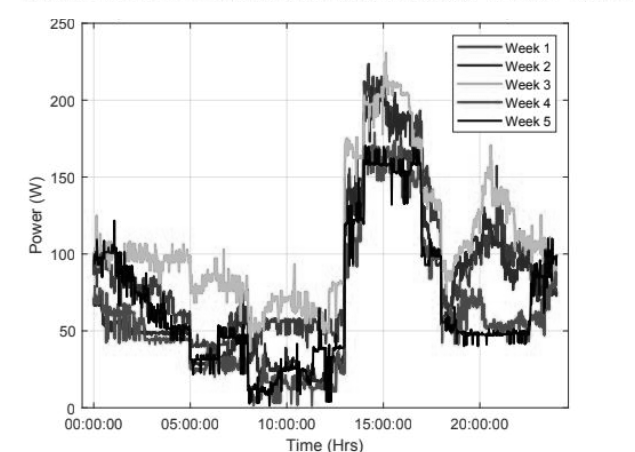
\includegraphics[width=0.65\textwidth]{loadcurve.png}
%\centering
%\caption{Five weeks monitored load curve from House 1.}
%\label{fig:loadcurve}
%\end{figure}
%
%\subsection{Experimental results}
%\label{sec:results}
%---------------------------------------------------
\section{Threats to Validity}
%---------------------------------------------------

This Chapter presented a favorable assessment of the proposed method. % over a diverse set of real-world benchmarks. 
Nevertheless, it also identified five threats to the validity of the results that bear further assessment.

\textit{Model precision:} each component of the PV system is mathematically modeled. %, and the precision of the proposed method depends on the precision of that particular model. 
The adoption of more complex models, or even an evaluation in a PV laboratory to validate the model could add more reliability to the results.

\textit{Time step:} The run-time complexity of the proposed method is an issue; the time step of one hour could be further reduced to approximate the algorithm to the real-world scenario.

\textit{Case studies:} The case studies were conducted in only  one municipality. A more complete evaluation can be done with more case studies.

\textit{Simulation Tool:} Only HOMER Pro was used. The inclusion of other specialized simulation tools or even a general simulation tool that uses the same mathematical model adopted by the automated verification could change the comparison.

\textit{Temperature and Solar Irradiance Data}: Information relating to the temperature and solar irradiance of each case study, whether it is using simulation or formal verification, comes from databases available online~\cite{Temperature, Irradiance}. However, in view of the fact that riverside communities do not have weather stations, the data used in the present study comes from the municipality closest (Manaus in all the case studies), where stations regularly collect the data. Nevertheless, accuracy recommends the use of weather stations in each location.

\section{Conclusion}

This Chapter showed in details how the state-of-the-art computer science method of automated verification was adapted to be used in stand-alone solar PV systems in order to validate their behavior. Moreover, it was possible to illustrate the comparative differences in how the proposed method and the traditional method of simulation work.

Detailed diagrams, flowcharts and algorithms with pseudo-code were presented in support of the proposed work and to aid the understanding. Additionally, the assumptions adopted in relation to the automated verification and simulation software were listed.

Furthermore, in this Chapter verifiers with the proposed automated verification using model checking were compared, which demonstrated that 'incremental' ESBMC had the best overall performance. CBMC presented the same results, but with a worse time to result, and CPAchecker was not conclusive (house $1$, house $2$, house $3$, and house $4$) because the \textit{time out} was not enough to obtain a result.

A comparison with a specialized simulation tool was also performed, although some of the tool's limitations, mainly related to not allow allowing battery autonomy setup or oversizing the battery bank by HOMER Pro, restricted the comparison between automated verification tools and simulation tools.

Based on the fact that all case studies were deployed in the field, with regular visits to conduct interviews with the residents, and with monitoring systems in some of the houses (house $1$, house $2$, house $3$, and house $4$), it was possible to compare the computational validation (by simulation or automated verification) with the real world employment of stand-alone solar PV systems. The final conclusion was that the proposed tool is sound and has an acceptable performance. 
